\clearpage % Rozdziały zaczynamy od nowej strony.

\section{Analiza wymagań systemu}

Przed rozpoczęciem implementacji systemu należy go przeanalizować pod kątem wymagań funkcjonalnych oraz niefunkcjonalnych. Twórca powinien uprzednio poznać występujące rodzaje danych, udostępniane na nich operacje oraz klasy użytkowników.

W systemach o architekturze mikroserwisowej należy również odpowiednio wydzielić serwisy, stanowiące spójną całość.

W tym rozdziale zostaną też przedstawione najważniejsze terminy i pojęcia używane w aplikacji, jej wymagania funkcjonalne i niefunkcjonalne.

\subsection{Słownik dziedziny problemu}

Słownik najważniejszych pojęć występujących w dziedzinie systemu. W nawiasach podano ich angielskie odpowiedniki, ponieważ w takiej formie zostały one użyte w kodzie aplikacji.

\begin{itemize}

    \item \textbf{Użytkownik zamawiający} (ang. \textit{Ordering User}) - encja reprezentująca użytkownika systemu, odpowiedzialnego za składanie zamówień. Użytkownik taki może definiować swoje adresy dostawy, oraz posiadać historię zamówień. Jest on definiowany przez nazwę oraz adres e-mail.
    \item \textbf{Restauracja} (ang. \textit{Restaurant}) - encja reprezentująca restaurację, która może być obsługiwana przez system. Restauracja posiada menu, które może być modyfikowane przez managera restauracji. Restauracja może być otwarta lub zamknięta, a jej manager może przyjmować lub odrzucać zamówienia. Restauracja jest definiowana przez nazwę, adres, menu oraz managera.
    \item \textbf{Kurier} (ang. \textit{Courier}) - encja reprezentująca dostawcę, który może być przypisany do zamówienia. Kurier może być dostępny lub niedostępny, a jego status może być aktualizowany samodzielne. Posiada on również lokalizację w postaci współrzędnych geograficznych. Kurier jest definiowany przez nazwę, adres e-mail oraz status.
    \item \textbf{Dostawa} (ang. \textit{Order Delivery}) - encja reprezentująca dostawę zamówienia przez kuriera z restauracji do użytkownika. Dostawa posiada status, który może być aktualizowany przez system. Dostawa jest definiowana przez zamówienie, kuriera, lokalizację restauracji, lokalizację użytkownika, obliczoną opłatę dla kuriera oraz status.
    \item \textbf{Zamówienie} (ang. \textit{Order}) - encja reprezentująca zamówienie użytkownika. Zamówienie posiada status, który może być aktualizowany przez system. Zamówienie jest definiowane przez użytkownika, restaurację, adres dostawy, listę dań oraz status.
    \item \textbf{Faktura} (ang. \textit{Invoice}) - encja reprezentująca fakturę wystawioną przez system. Faktura może być wystawiona dla użytkownika, restauracji lub kuriera. Faktura jest definiowana przez składniki, kwotę, datę wystawienia oraz adres e-mail odbiorcy.
    \item \textbf{Płatność} (ang. \textit{Order Payment}) - encja reprezentująca płatność za zamówienie. Płatność może być dokonana przez użytkownika. Płatność jest definiowana przez zamówienie, metodę płatności, kwotę oraz status.
    \item \textbf{Odbiora płatności} (ang. \textit{Payee}) - encja reprezentująca odbiorcę płatności. Odbiorca płatności może być restauracją lub kurierem. Odbiorca płatności jest definiowany przez nazwę, adres e-mail oraz balans kwotowy.
    \item \textbf{Płatnik} (ang. \textit{Payer}) - encja reprezentująca płatnika. Płatnik może być użytkownikiem lub systemem. Płatnik jest definiowany przez nazwę oraz adres e-mail.
    \item \textbf{Zamówienie restauracyjne} (ang. \textit{Restaurant Order}) - encja reprezentująca zamówienie złożone w restauracji. Zamówienie restauracyjne posiada status, który może być aktualizowany przez system. Zamówienie restauracyjne jest definiowane przez restaurację, listę dań oraz status.

\end{itemize}

\subsection{Burza Zdarzeń}

Aby móc podzielić system informatyczny na komponenty, później przekształcone w mikroserwisy, można zastosować np. technikę Burzy Zdarzeń (ang. Event Storming \cite{eventstorming}.

Burza Zdarzeń to metoda warsztatowa używana w projektowaniu i analizie systemów opartych na mikroserwisach. Została opracowana przez Alberto Brandoliniego i polega na interaktywnym modelowaniu procesów biznesowych poprzez identyfikację i dyskusję na temat "zdarzeń" mających znaczenie biznesowe. Uczestnicy, wykorzystując kolorowe karteczki, reprezentują różne aspekty systemu, takie jak wydarzenia, komendy, czy modele danych. Ta metoda sprzyja współpracy między różnymi zespołami, pomagając im lepiej zrozumieć procesy biznesowe i technologiczne oraz identyfikować potencjalne problemy i możliwości dla architektury mikroserwisowej.

\begin{figure}[!h]
    \centering 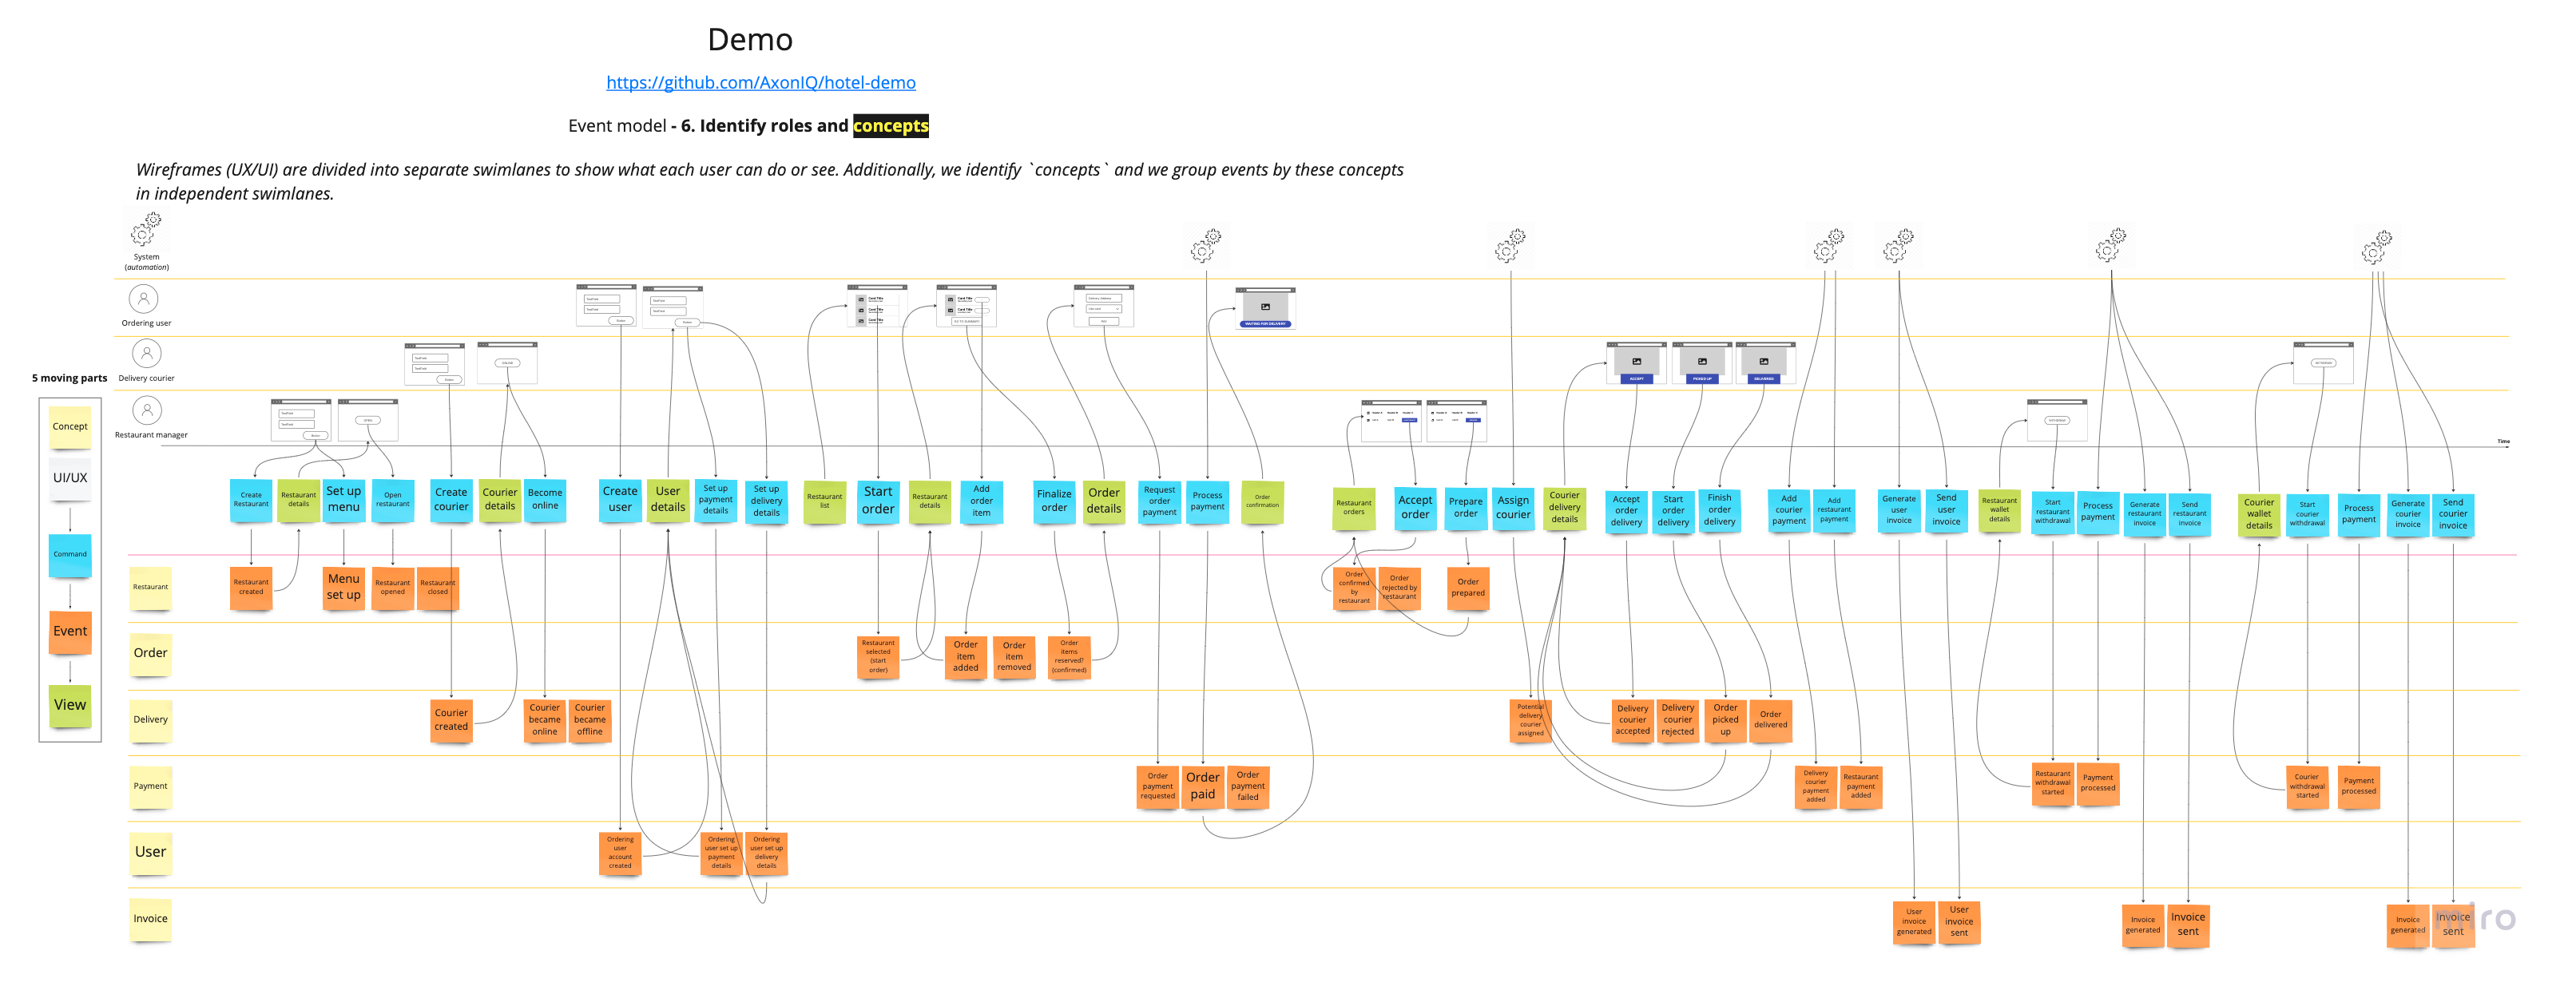
\includegraphics[width=1.0\linewidth]{event_storming.png}
    \caption{Przykładowy rezultat sesji Burzy Zdarzeń \cite{event_storming_rys}}
\end{figure}


Rezultatem sesji Burzy Zdarzeń powinna być lista zdarzeń zgrupowanych w ramach tzw. agregatów dziedzinowych, czyli obiektów realizujących konkretny zbiór logiki biznesowej. W tej postaci łatwo postawić granice między słabo powiązanymi grupami agregatów. Zbiór agregatów po jednej stronie granicy nazywamy Ograniczonym Kontekstem (ang. Bounded Context \cite{boundedcontext})). Są to kandydaci do wydzielenia jako mikroserwisy modelowanej aplikacji.

W ramach pracy inżynierskiej przeprowadzono dla projektowanego systemu sampdzielną sesję Burzy Zdarzeń z wykorzystaniem narzędzia Miro.

Miro \cite{miro} to interaktywna platforma webowa, umożliwiająca tworzenie tablic z notatkami, rysunkami i diagramami. Wybór tego narzędzia był podyktowany jego prostotą użytkowania oraz możliwościami wizualizacji efektów.

W ramach sesji przeprowadzono kolejno następujące kroki:

\begin{itemize}

    \item \textbf{Definicja zdarzeń biznesowych}: Zidentyfikowano kluczowe zdarzenia w procesie biznesowym i zapisuno je na karteczkach (np. "zamówienie złożone", "płatność przyjęta").
    \item \textbf{Układanie zdarzeń}: Zdarzenia zostały ułożone w kolejności chronologicznej, tworząc w ten sposób proces biznesowy.
    \item \textbf{Identyfikacja komend}: Zidentyfikowano komendy, które mogą wywołać zdarzenia (np. "złóż zamówienie").
    \item \textbf{Identyfikacja modeli}: Zidentyfikowano modele danych, które są potrzebne do realizacji procesu biznesowego (np. "zamówienie").
    \item \textbf{Identyfikacja agregatów}: Zidentyfikowano agregaty dziedzinowe, czyli grupy powiązanych ze sobą zdarzeń, komend i modeli danych (np. "zamówienie").
    \item \textbf{Identyfikacja ograniczonych kontekstów}: Zidentyfikowano ograniczone konteksty, czyli grupy powiązanych ze sobą agregatów dziedzinowych (np. "zamówienie").
    \item \textbf{Identyfikacja widoków}: Zidentyfikowano widoki, czyli dane, które są potrzebne do wyświetlenia w interfejsie użytkownika (np. "lista restauracji").

\end{itemize}

\clearpage

\begin{figure}[!h]
    \centering 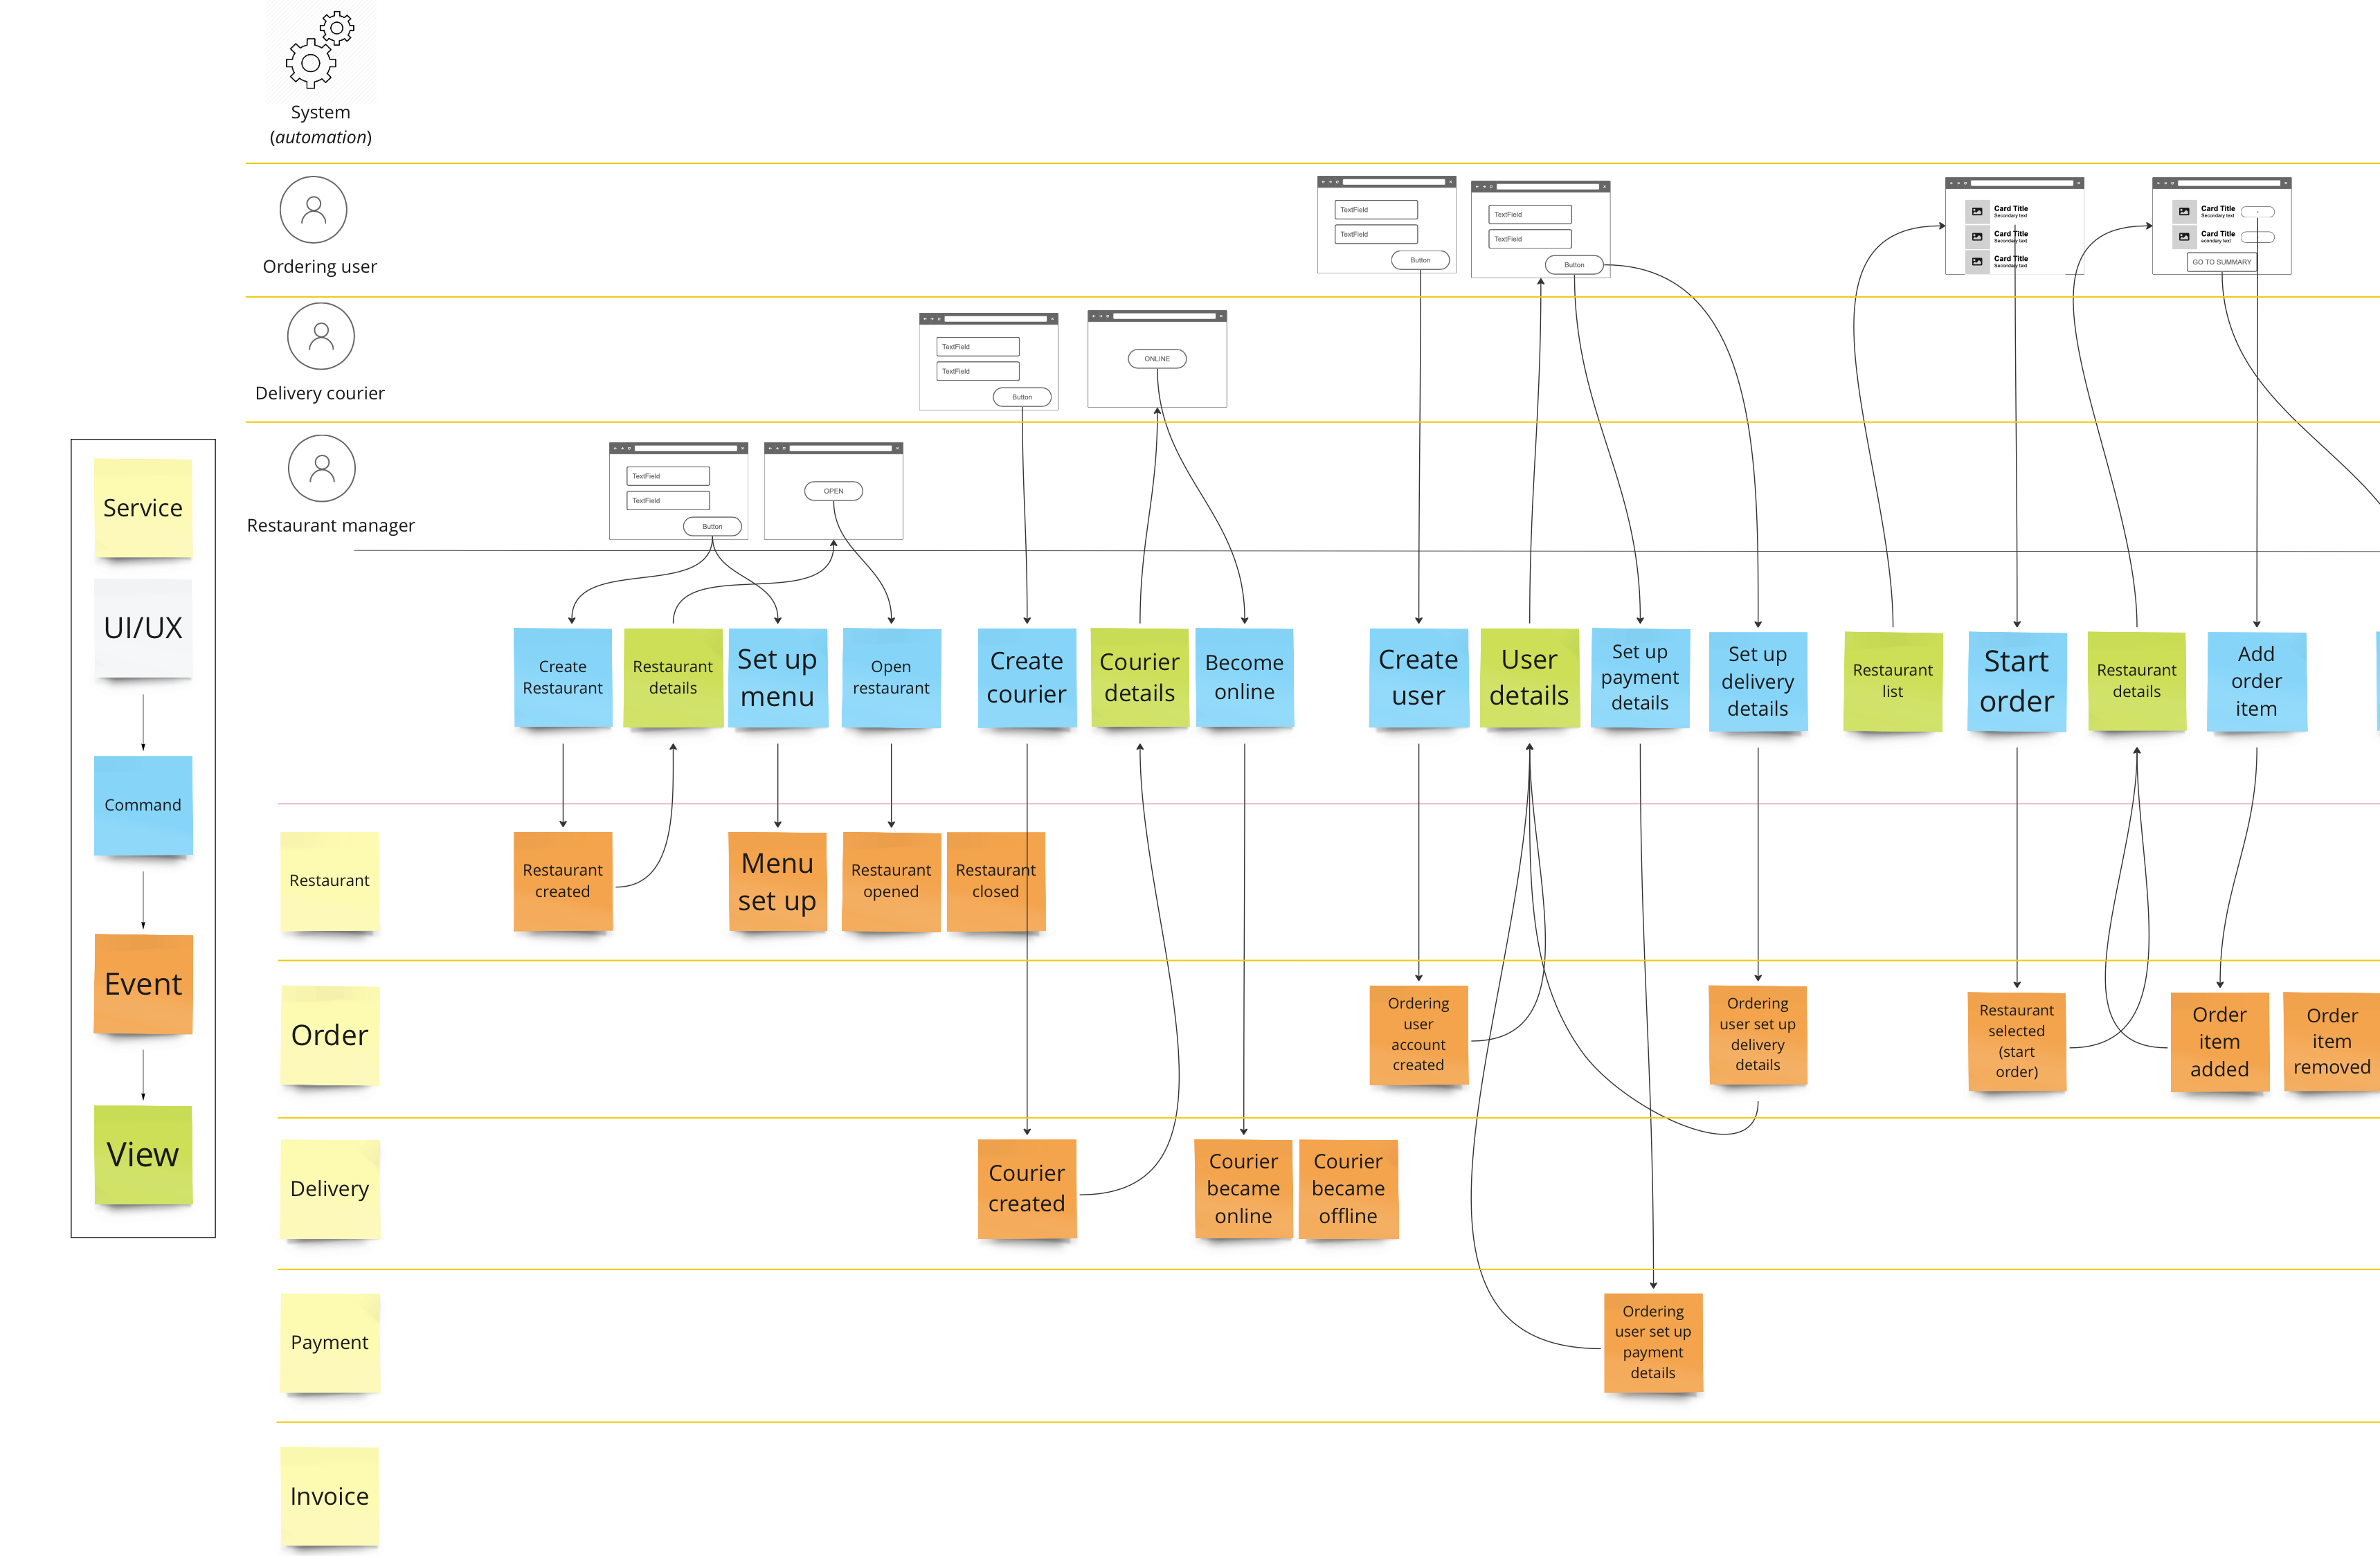
\includegraphics[width=1.0\linewidth]{event_storming2.png}
    \caption{Rezultat sesji Burzy Zdarzeń dla projektowanego systemu}
\end{figure}

\subsection{Identyfikacja Ograniczonych Kontekstów}

W wyniku sesji Burzy Zdarzeń zidentyfikowano pięć kontekstów granicznych, które będą kluczowe dla tworzonej aplikacji. Są to:

\textbf{Restaurant} (\textit{Restauracja}) - obejmuje zarządzanie restauracjami, menu oraz definicją i dostępnością produktów. Potrafi wyliczyć aktualną cenę produktów w zamówieniu oraz zwalidować ich dostępność,

\textbf{Order} (\textit{Zamówienie}) - odpowiada za proces zamówienia, jego składanie, modyfikowanie, anulowanie oraz koordynuje cały proces przygotowania zamówienia do momentu dostawy. Umożliwia również zarządzanie danymi użytkowników i ich adresami dostaw,

\textbf{Delivery} (\textit{Dostawa}) - koncentruje się na logistyce dostaw, monitorowaniu statusu dostawy oraz komunikacji z dostawcą. Zarządza również bazą dostawców i ich lokalizacjami. Odpowiada za proces dopasowania dostawcy do zamówienia,

\textbf{Payment} (\textit{Płatność}) - zarządza procesem płatności, obejmuje różne metody płatności oraz obsługę transakcji. Obsługuje wszelkie rozliczenia w ramach systemu. Odpowiada również za generowanie faktur dla użytkowników, restauracji i dostawców i ich wysyłkę,

\medskip

Powyższe cztery konteksty stały się podstawą do wydzielenia mikroserwisów w ramach projektowanego systemu. Każdy z nich będzie realizowany przez osobny komponent.

\subsection{Wymagania funkcjonalne}

Wymagania funkcjonalne zostały zidentyfikowane na podstawie komend i zdarzeń, które zostały wylistowane w ramach sesji Burzy Zdarzeń. Są to, z podziałem na klasy użytkowników:

\medskip

\textbf{Jako użytkownik zamawiający}
\begin{itemize}
    \item mogę utworzyć konto w systemie,
    \item mogę uwierzytelnić się przy pomocy loginu i hasła lub konta Google,
    \item mogę dodać detale dostawy,
    \item mogę wylistować restauracje wraz z ich średnią oceną,
    \item mogę rozpocząć proces zamówienia wybierając restaurację,
    \item mogę wybrać dania z menu i dodać je do zamówienia,
    \item mogę złożyć zamówienie,
    \item mogę opłacić zamówienie przy użyciu zewnętrznej bramki płatności,
    \item mogę śledzić status zamówienia,
    \item mogę wylistować historyczne zamówienia,
    \item mogę otrzymać fakturę za zamówienie na podany adres e-mail.
\end{itemize}

\medskip

\textbf{Jako manager restauracji}
\begin{itemize}
    \item mogę utworzyć konto restauracji w systemie,
    \item mogę uwierzytelnić się przy pomocy loginu i hasła lub konta Google,
    \item mogę zaktualizować detale i dostępność (otwarta/zamknięta) restauracji,
    \item mogę skonfigurować menu restauracji,
    \item mogę wylistować zamówienia będące w trakcie,
    \item mogę wylistować zamówienia historyczne,
    \item mogę przyjąć zamówienie do realizacji,
    \item mogę odrzucić zamówienie,
    \item mogę oznaczyć zamówienie jako gotowe,
    \item mogę wypłacić środki za zamówienia na podany numer konta,
    \item mogę otrzymać fakturę za zamówienie na podany adres e-mail.
\end{itemize}

\medskip

\textbf{Jako dostawca}
\begin{itemize}
    \item mogę utworzyć konto w systemie,
    \item mogę uwierzytelnić się przy pomocy loginu i hasła lub konta Google,
    \item mogę zaktualizować swój status (dostępny/niedostępny),
    \item mogę zobaczyć dostępną ofertę dostawy,
    \item mogę przyjąć albo odrzucić ofertę dostawy,
    \item mogę zaktualizować status dostawy (odebrana z restauracji, dostarczona do użytkownika),
    \item mogę wylistować historyczne dostawy,
    \item mogę wypłacić środki za dostarczone zamówienia na podany numer konta,
    \item mogę otrzymać fakturę za dostarczone zamówienia na podany adres e-mail.
\end{itemize}

\subsection{Wymagania niefunkcjonalne}

Wymagania niefunkcjonalne zostały zidentyfikowane m.in. na podstawie ograniczeń biznesowych, wymagań funkcjonalnych oraz doświadczenia Autora w budowaniu skalowalnych aplikacji webowych. Ponadto zostały one zainspirowane listą 12 czynników wpływających na jakość oprogramowania zaproponowaną przez Adama Wigginsa \cite{12factors}.

\textbf{Skalowalność} - każdy z komponentów systemu powinien być skalowalny poziomo w zależności od obciążenia. Każdy mikroserwis powinien móc być replikowalny,

\textbf{Wydajność} - system powinien umożliwiać równoległe przetwarzanie minimum 50 dowolnych żądań HTTP na sekundę,

\textbf{Wysoka dostępność} - możliwość częściowej pracy pomimo utraty niektórych komponentów systemu. System powinien być odporny na awarie,

\textbf{Monitorowanie} - aplikacja powinna umożliwiać monitorowanie i logowanie zdarzeń w celu analizy i debugowania. Każdy mikroserwis powinien logować swoje zdarzenia w centralnym repozytorium, a system powinien umożliwiać monitorowanie stanu mikroserwisów.

\textbf{Testowalność} - system powinien być łatwy do testowania, zarówno jednostkowo jak i integracyjnie oraz wydajnościowo.

\textbf{Bezpieczeństwo} - aplikacja powinna zapewniać odpowiednie zabezpieczenia w celu ochrony poufności, integralności i dostępności danych. Dostęp do mikroserwisów powinien być chroniony przez autoryzację i uwierzytelnianie, a dane powinny być szyfrowane w tranzycie.

\textbf{Synchronizacja i spójność danych} - system powinien zapewniać ostateczną spójność danych pomiędzy mikroserwisami.